 \let\negmedspace\undefined
\let\negthickspace\undefined
\documentclass[journal]{IEEEtran}
\usepackage[a5paper, margin=10mm, onecolumn]{geometry}
%\usepackage{lmodern} % Ensure lmodern is loaded for pdflatex
\usepackage{tfrupee} % Include tfrupee package

\setlength{\headheight}{1cm} % Set the height of the header box
\setlength{\headsep}{0mm}     % Set the distance between the header box and the top of the text

\usepackage{gvv-book}
\usepackage{gvv}
\usepackage{cite}
\usepackage{amsmath,amssymb,amsfonts,amsthm}
\usepackage{algorithmic}
\usepackage{graphicx}
\usepackage{textcomp}
\usepackage{xcolor}
\usepackage{txfonts}
\usepackage{listings}
\usepackage{enumitem}
\usepackage{mathtools}
\usepackage{gensymb}
\usepackage{comment}
\usepackage[breaklinks=true]{hyperref}
\usepackage{tkz-euclide} 
\usepackage{listings}
% \usepackage{gvv}                                        
\def\inputGnumericTable{}                                 
\usepackage[latin1]{inputenc}                                
\usepackage{color}                                            
\usepackage{array}                                            
\usepackage{longtable}                                       
\usepackage{calc}                                             
\usepackage{multirow}                                         
\usepackage{hhline}                                           
\usepackage{ifthen}                                           
\usepackage{lscape}
\begin{document}

\bibliographystyle{IEEEtran}
\vspace{3cm}

\title{1.10.28}
\author{EE25BTECH11060 - V.Namaswi}
% \maketitle
% \newpage
% \bigskip
{\let\newpage\relax\maketitle}

\renewcommand{\thefigure}{\theenumi}
\renewcommand{\thetable}{\theenumi}
\setlength{\intextsep}{10pt} % Space between text and floats
\textbf{Question}:\\Write a unit vector in \textbf{XY} plane making an angle 30\degree with positive direction of \textbf{X} axis

\textbf{Solution}:\\Given a vector,\\
Angle made by the vector with X axis = 30\degree\\
Angle made by the vector with Y axis =90\degree-30\degree=60\degree\\
Angle made by the vector with Z axis =90\degree\\

\begin{table}[ht]
\centering
\begin{tabular}{|c|c|}
\hline
\textbf{Axis} & \textbf{Angle (in degrees)} \\
\hline
X-axis & 30\degree \\
Y-axis & 60\degree \\
Z-axis & 0\degree \\
\hline
\end{tabular}
\caption{Angles made by the X, Y, Z axes}
\end{table}

Unit vector is given by 
\begin{align*}
\implies
    \begin{myvec}{\cos30\degree\\\cos60\degree\\\cos90\degree}\end{myvec}\\
    \implies
    \begin{myvec}
       {\frac{\sqrt3}{2}\\\frac{1}{2}\\0}
    \end{myvec}
\end{align*}

The unit  vector of the given vector is given by
 $\frac{\sqrt{3}}{2}\,\mathbf{i} + \frac{1}{2}\,\mathbf{j}$



Refer Fig
\begin{figure}
    \centering
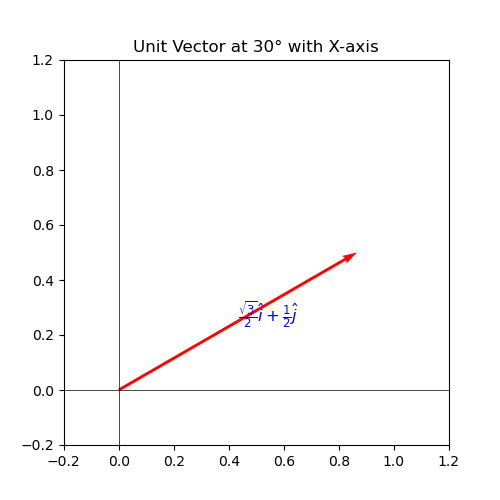
\includegraphics[width=0.8\columnwidth]{figs/Figure _2.png}
    \caption{Plot}
    \label{fig:placeholder}
\end{figure}
\end{document}